%\section{Distortion Correction with Conditionals}
\Echapter{Distortion Correction with Conditionals}{Dan Peterson}{djpeters@uw.edu}

In this example, we will use a makefile to apply the appropriate distortion correction procedure automatically, utilizing conditionals.

First, a bit of background: The most common way to take a series of MRI images as quickly as possible is to use what is called an ``echo-planar imaging readout,'' or ``EPI.'' A drawback that comes with this rapid acquisition is that EPI images are prone to distortions due to an uneven magnetic field. Sometimes these distortions are called ``susceptibility-induced distortions,'' because it is the differing magnetic susceptibility of tissue, bone, and air that causes the magnetic field to be uneven. Fortunately, since these distortions are constant and predictable within an imaging session, they can be un-done.

We will consider two ways of undoing these distortions, each requiring at least one extra image to be acquired. The first method is to acquire an image of the uneven magnetic field, called a ``fieldmap.'' This image contains a map of the deviation from the main magnetic field, in radians/sec (the resonance frequency of the water protons is directly proportional to the strength of the magnetic field as per the Larmor equation: $\omega=\gamma B _{0}$). To do this we will use a tool called \texttt{fugue}, which is distributed as part of FSL. \texttt{fugue} will convert this fieldmap into a nonlinear warp, and then we can apply that warp to undo the susceptibility-induced distortions. The other method is to acquire an additional image with the EPI readout going in the other direction, meaning that the direction of the susceptibility-induced distortion will be reversed. We can then use a tool called \texttt{topup} (also from FSL), that will warp two images with opposite distortions towards each other, until they meet in the middle. We can then apply this computed warp to the rest of our data.

These are two different procedures that require different sets of files (an acquisition parameters fire for \texttt{topup} and a fieldmap for \texttt{fugue}), but can be part of an otherwise similar pipeline. We can use \maken{} to sense which procedure to use based on what files are present, and assemble the appropriate prerequisites.

In order to be very clear about the behavior of \maken{}, below is an example of a ``toy'' makefile, which does not call any real programs, and can operate on empty ``dummy'' files. When debugging and developing makefiles it can be useful to write such simplified makefiles, and run them with \maken{}\texttt{-n}.

\begin{lstlisting}
	%*\lnote*SDC_METHOD = $(shell if [ -f fieldmap ] ; then echo FUGUE; \
					elif [ -f acqparams ] ; then echo TOPUP; \
					else echo FALSE ; fi)

	motion_corrected_dataset: raw_diffusion_dataset
		toy_eddy raw_diffusion_dataset

	topup_result: raw_diffusion_dataset acqparams
		toy_topup raw_diffusion_dataset acqparams

	%*\lnote*ifeq ($(SDC_METHOD),TOPUP)

	fully_corrected_diffusion_dataset: raw_diffusion_dataset topup_result
		toy_eddy raw_diffusion_dataset topup_result

	else ifeq ($(SDC_METHOD),FUGUE)

	fully_corrected_diffusion_dataset: motion_corrected_dataset fieldmap
		toy_fugue motion_corrected_dataset fieldmap

	else
	%*\lnote*$(error ERROR: neither fieldmap for FUGUE \
						nor acquisition parameter file for TOPUP were found)
	endif

	tensor: fully_corrected_diffusion_dataset
		toy_solve_tensor fully_corrected_diffusion_dataset
\end{lstlisting}

\lnum{1} If there is a file called \texttt{fieldmap} in the working directory we want to use \texttt{fugue}, and if \texttt{acqparams} exists instead, we want to use \texttt{topup}. \\
\indent \lnum{2} When \maken{} runs, it will insert a different recipe into the set of rules depending on the value of \texttt{SDC_METHOD}. The conditional block extends until \texttt{endif}. The \texttt{else ifeq} statement in the middle is part of the same conditional block (i.e. you only need one \texttt{endif}).\\
\indent \lnum{3} It's always a good idea to halt and raise an error if none of the expected conditions are met.

If we run this makefile to build the \texttt{tensor} target (using the \texttt{-n} flag) in a directory that contains both \texttt{raw_diffusion_dataset} and \texttt{fieldmap}, the result looks like this:
\bashcmd{make -n tensor \\toy_eddy raw_diffusion_dataset \\toy_fugue motion_corrected_dataset fieldmap \\toy_dtifit fully_corrected_diffusion_dataset}

However, if both \texttt{raw_diffusion_dataset} and \texttt{acqparams} (and not \texttt{fieldmap}) are in the directory, we see:
\bashcmd{make -n tensor \\toy_topup raw_diffusion_dataset acqparams \\toy_eddy raw_diffusion_dataset topup_result \\toy_dtifit fully_corrected_diffusion_dataset}

The toy makefile is visualized in a flowchart in \autoref{toy-example}.

\begin{figure}
	\begin{center}  % not necessary, but usually preferred.
		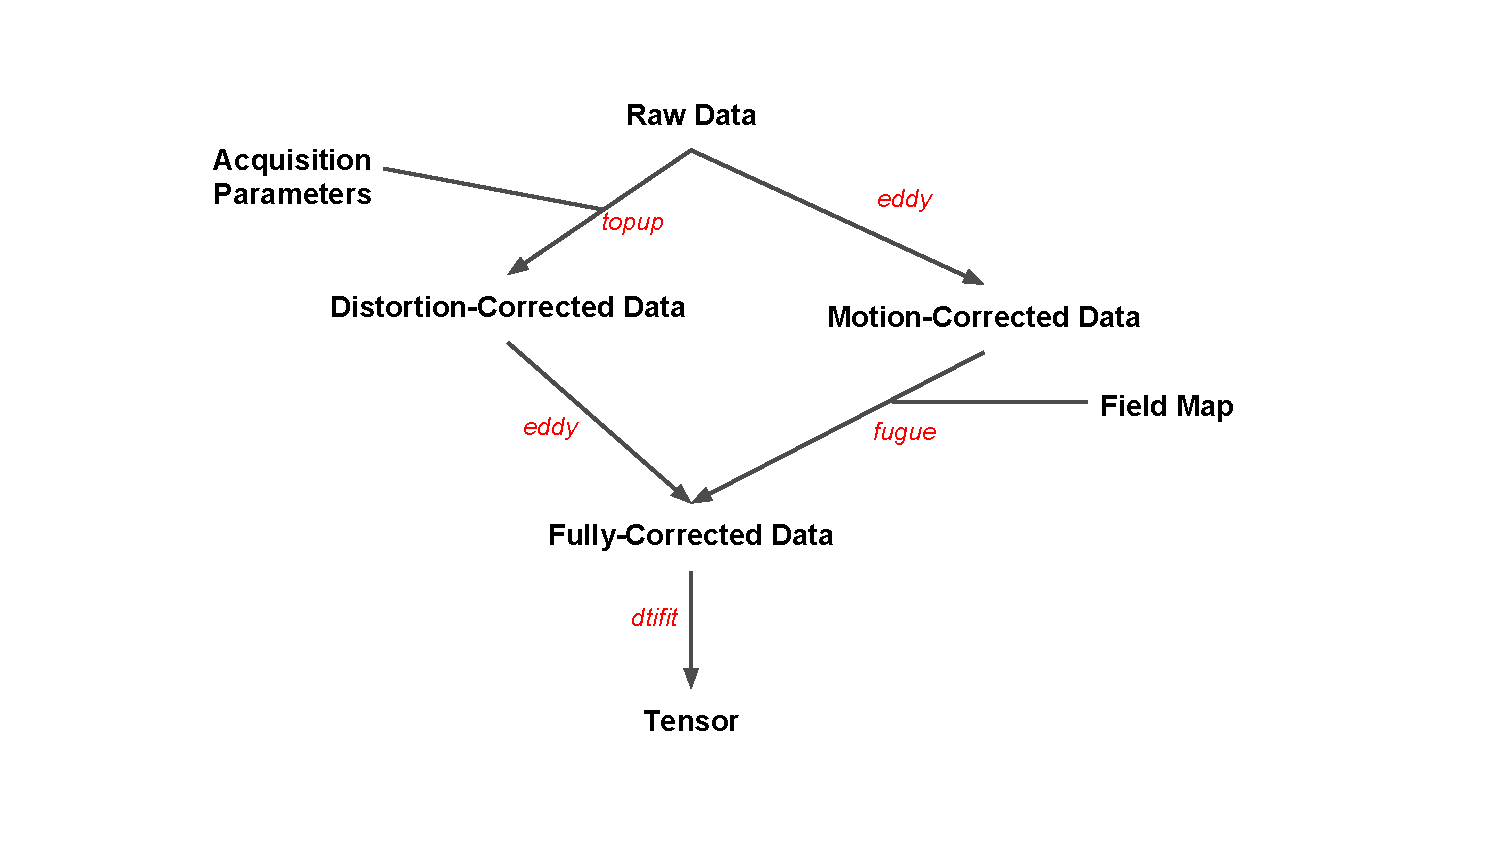
\includegraphics[width=\textwidth]{images/distcorr-flowchart.pdf}
	\end{center}
	\label{toy-example}
	\caption{Toy Makefile}
\end{figure}


If we were to implement this process in a bash script, the earlier ``upstream'' processes would need to be part of the conditional block. An advantage of using \maken{} for workflows is that \textit{only} the part that causes the ``split'' in the branching logic needs to be surrounded by the if-then-else-end logic. Also note that if we were using \texttt{topup} with a fieldmap, but for some reason we wanted to do just the motion correction (like for QC, or for debugging purposes), that unused ``branch'' of the makefile would be available with a simple \texttt{make motion_corrected_dataset} command. 

Here's the full Makefile:

\begin{lstlisting}
	ifeq "$(origin MAKEPIPELINES)" "undefined"
	MAKEPIPELINES=/project_space/makepipelines
	endif

	# Uncomment and set this to be the location of FSL in your environment
	# FSL_DIR=/usr/share/fsl/5.0

	# Set this to be 1 if you intend to parallelize using make. Otherwise
	# eddy will use all cores available on your machine. 
	# export OMP_NUM_THREADS=1

	PROJECT_DIR=$(MAKEPIPELINES)/dti_suceptibility_correction

	SDC_METHOD = $(shell if [ -f fieldmap.nii.gz ] ; then echo FUGUE; \
	                    elif [ -f acqparams.txt ] ; then echo TOPUP; \
	                    else echo FALSE ; fi)

	#for some reason fslval returns a trailing space, which tr deletes
	NUM_DIFFUSION_VOLS =$(shell fslval raw_diffusion.nii.gz dim4 | tr -d '\040\011\012\015')

	# default is 4
	EDDY_ITERATIONS = 1

	# fast, or accurate
	TOPUP_MODE=fast

	ECHO_SPACING =.00072
	UNWARP_DIRECTION=y-

	.PHONY: clean tensor

	# just motion-correct using eddy
	# creates a dummy acqparams and index file (eddy requires that you supply them), then deletes them
	mec_diffusion.nii.gz: raw_diffusion.nii.gz bval bvec brain_mask.nii.gz
		echo "0 1 0 0.072" > temp_acqparams.txt ;\
		for i in `seq 1 $(NUM_DIFFUSION_VOLS)`; do echo 1 >> temp_index.txt ; done ;\
		eddy --imain=raw_diffusion.nii.gz --mask=brain_mask.nii.gz --index=temp_index.txt --acqp=temp_acqparams.txt --bvecs=bvec --bvals=bval --out=mec_diffusion --niter=$(EDDY_ITERATIONS) --verbose  ;\
		rm temp_acqparams.txt temp_index.txt

	# suceptibility distortion correction with topup from a blip-up, blip-down acquisition
	# 	take the two B0s out of the diffusion dataset
	# 	run topup to estimate suceptibility distortions using the two B0s
	topup_results_movpar.txt: raw_diffusion.nii.gz acqparams.txt
		fslroi raw_diffusion.nii.gz S0_images.nii.gz 0 2 ;\
		topup --imain=S0_images --datain=acqparams.txt --config=$(PROJECT_DIR)/lib/b02b0_$(TOPUP_MODE).cnf --out=topup_results --fout=field_est --iout=unwarped_S0_images --verbose

	ifeq ($(SDC_METHOD),TOPUP)

	# using eddy, simultaneously correct for motion and apply the result from topup
	sdc_mec_diffusion.nii.gz: raw_diffusion.nii.gz topup_results_movpar.txt index.txt
		eddy --imain=raw_diffusion.nii.gz --mask=brain_mask --acqp=acqparams.txt --index=index.txt --bvecs=bvec --bvals=bval --topup=topup_results --out=sdc_mec_diffusion.nii.gz --niter=$(EDDY_ITERATIONS) --verbose

	else ifeq ($(SDC_METHOD),FUGUE)

	# use fugue to correct a dataset for suceptibility distortions that has already been corrected for moton and eddy currents
	sdc_mec_diffusion.nii.gz: mec_diffusion.nii.gz fieldmap.nii.gz
		fugue --loadfmap=fieldmap.nii.gz --dwell=$(ECHO_SPACING) -i mec_diffusion.nii.gz -u sdc_mec_diffusion.nii.gz --unwarpdir=$(UNWARP_DIRECTION) -v

	else
	$(error ERROR: neither fieldmap for FUGUE nor acquisition parameter file for TOPUP were found)
	endif

	# solve tensor from fully corrected data set
	tensor: sdc_mec_diffusion.nii.gz brain_mask.nii.gz bvec bval
		dtifit -k sdc_mec_diffusion.nii.gz -r bvec -b bval -m brain_mask -o dti

clean:
		rm -f dti_* sdc_mec_diffusion.* mec_diffusion.* S0_images* field_est.nii.gz topup_results* unwarped_S0_images.nii.gz

	# Left as as excercise to the reader:
	# - unwarp brain mask
	# - coregister fieldmap to DTI
	# - adjust bvecs for motion correction

\end{lstlisting}

There are a few more files and commands here than in the toy example, but the basic structure is the same. It's still missing some elements of a full-featured DTI preprocessing pipelines, but this example illustrates how using conditional statements in makefiles can make them more robust and versatile. \break

More information about the options and the formats of the files supplied to \texttt{eddy}, \texttt{topup}, and \texttt{fugue} is available on the FSL website (\url{http://fsl.fmrib.ox.ac.uk/fsl/fslwiki/FslOverview})

